\section{Methodology}

IT HAS 8K keys!

%\begin{figure*}[tbh]
%  \noindent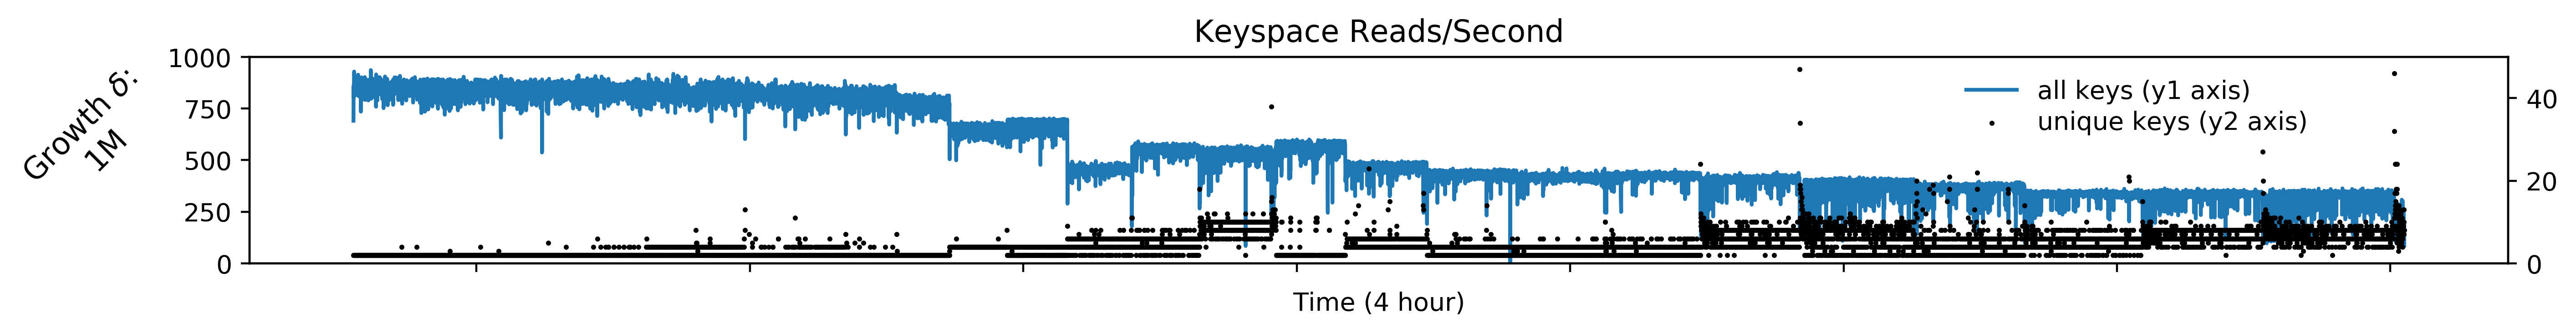
\includegraphics[width=1\textwidth]{figures/keyspace-regimes-4hr.png}\\
%  \caption{Access patterns for a growth \(\delta\) of 1M shows similiar
%  behavior to 100K but on different time scales.
%  \label{fig:keyspace-regimes-4hr}}
%\end{figure*}

\subsection{Contribution 1: ParSplice Keyspace Analysis}
Part 2: As Parsplice simulates, entropy increases resulting in keyspace
inbalance (Figure~\ref{fig:keyspace-regimes} shows how imbalance controlled by
``growth rate")


\begin{figure}[tbh]
  \noindent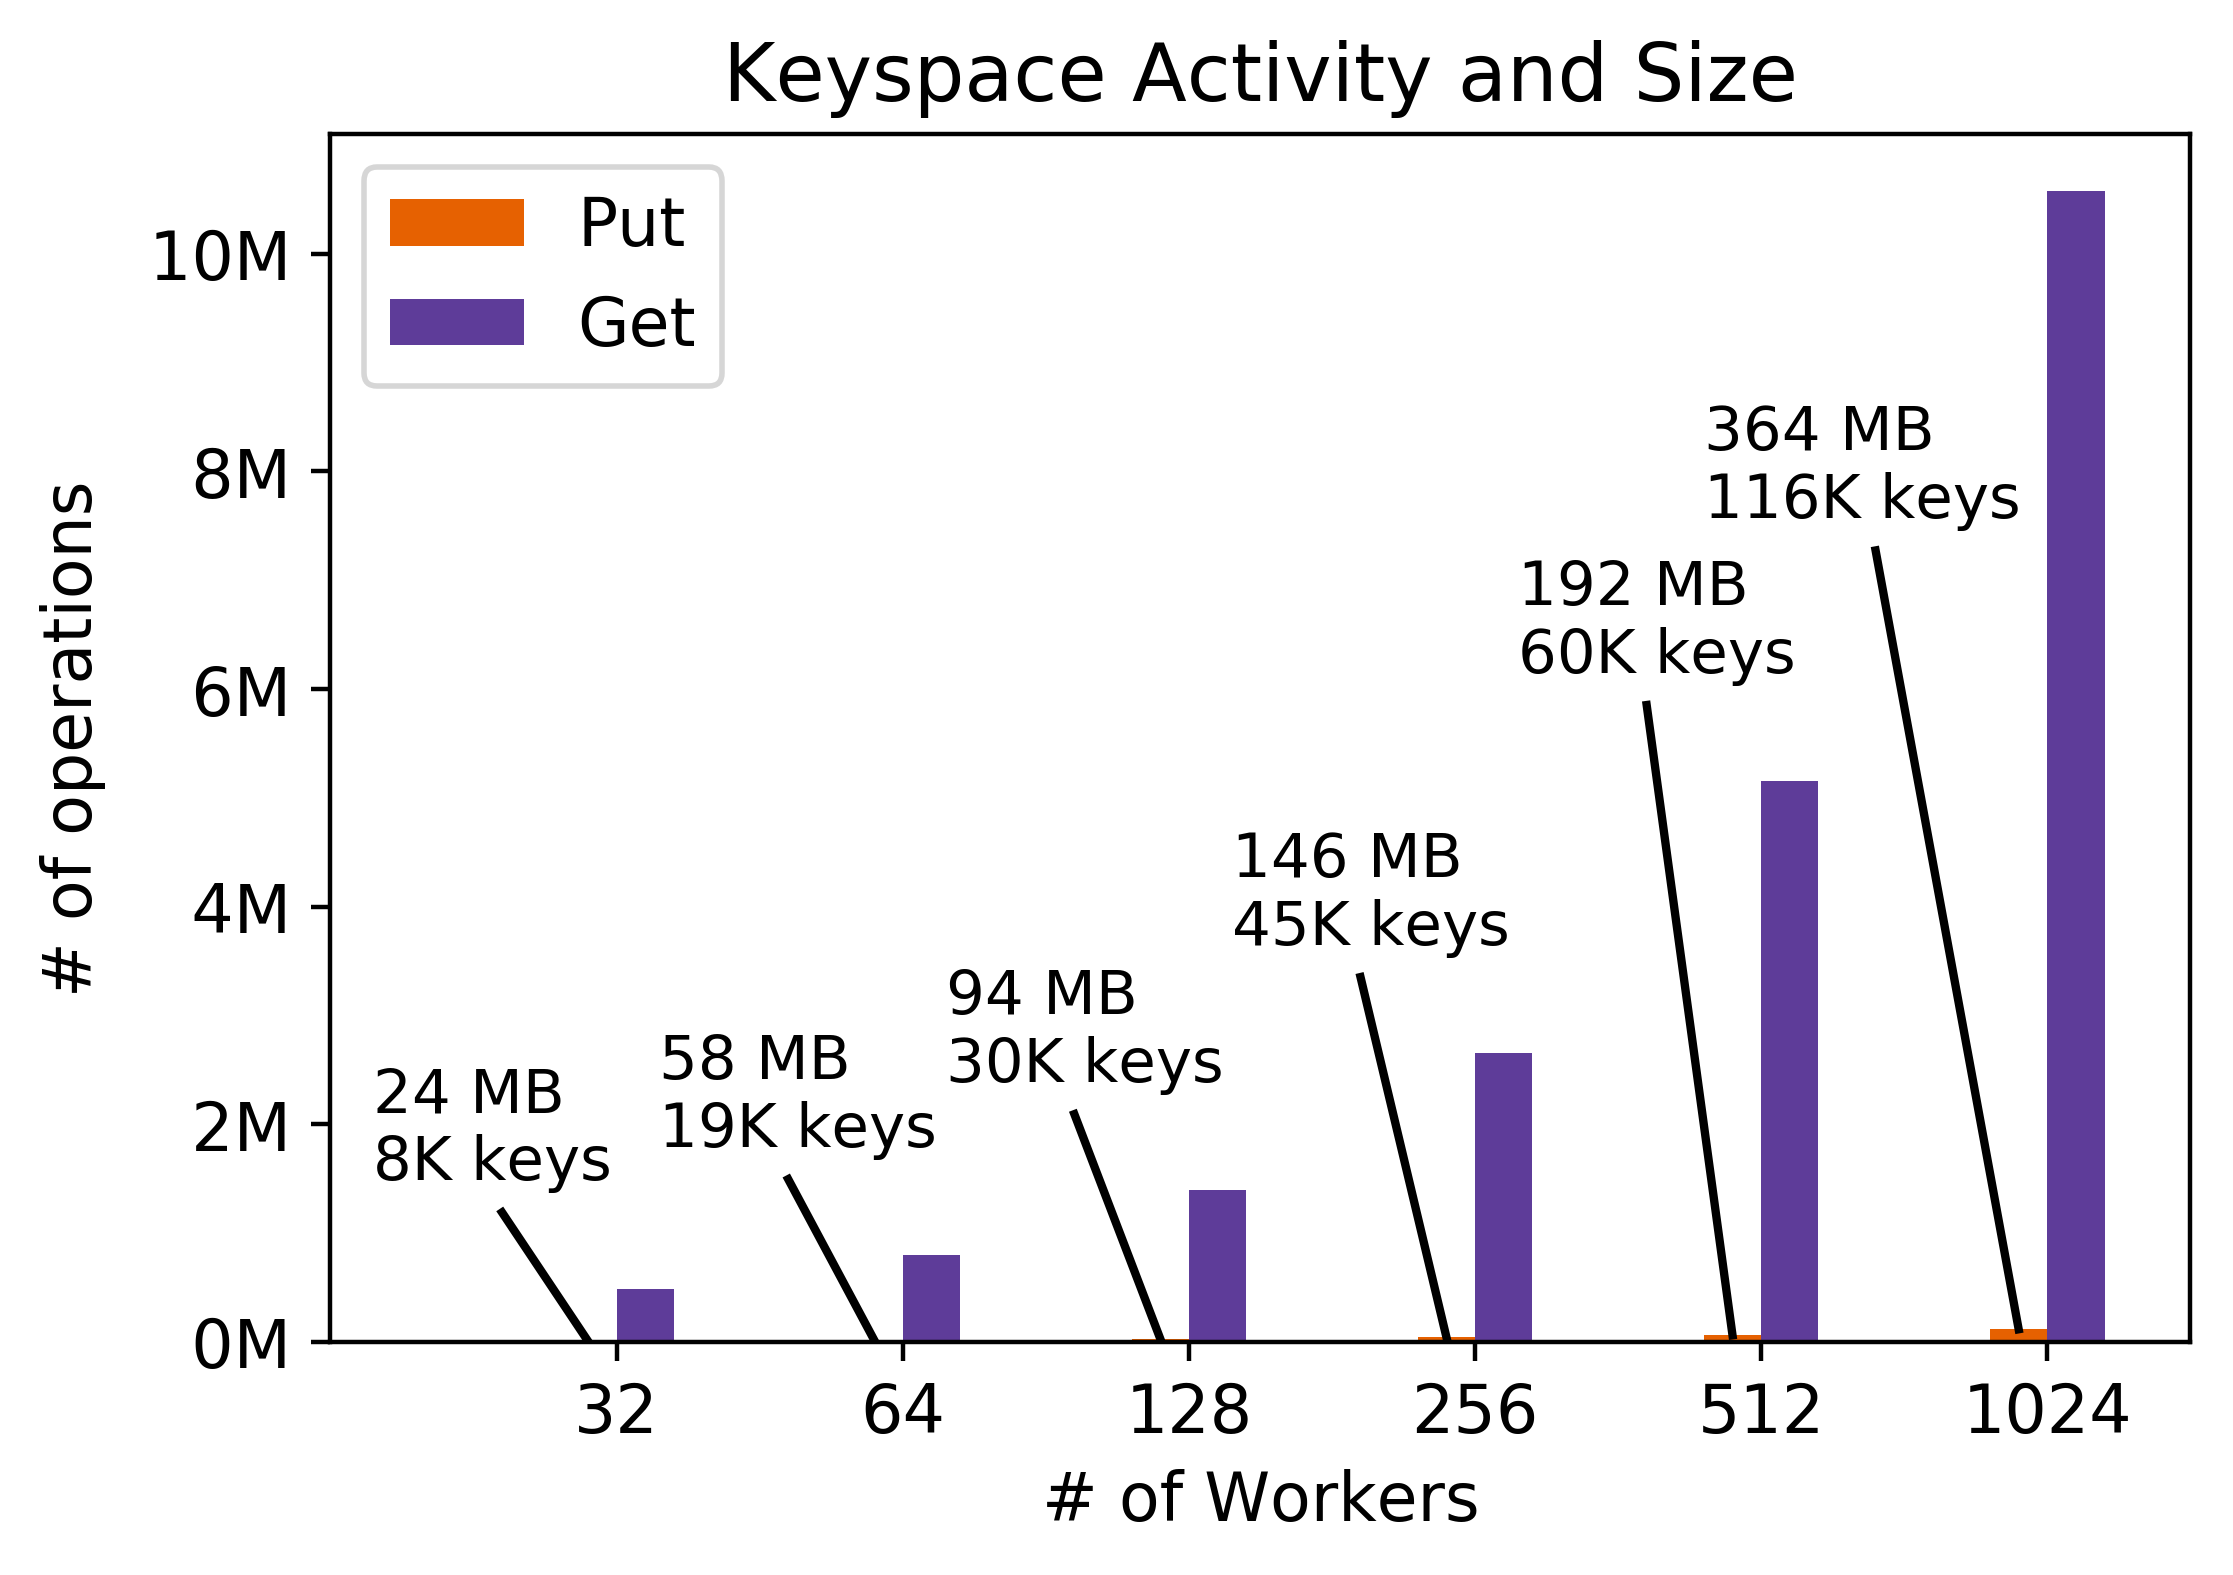
\includegraphics[width=0.5\textwidth]{figures/methodology-keyspace.png}\\
  \caption{ The ParSplice keyspace is small (numbers above bars) but must
  satisfy many reads as workers calculate new segments. The active keyspace is
  difficult to predict a priori but the optimal load balancing strategy strikes a
  good balance between preformance and utiization. 
  \label{fig:methodology-keyspace}}
\end{figure}

\subsection{Contribution 2: Positive Effects of Load Balncing}
  \begin{figure}[tbh]
  \noindent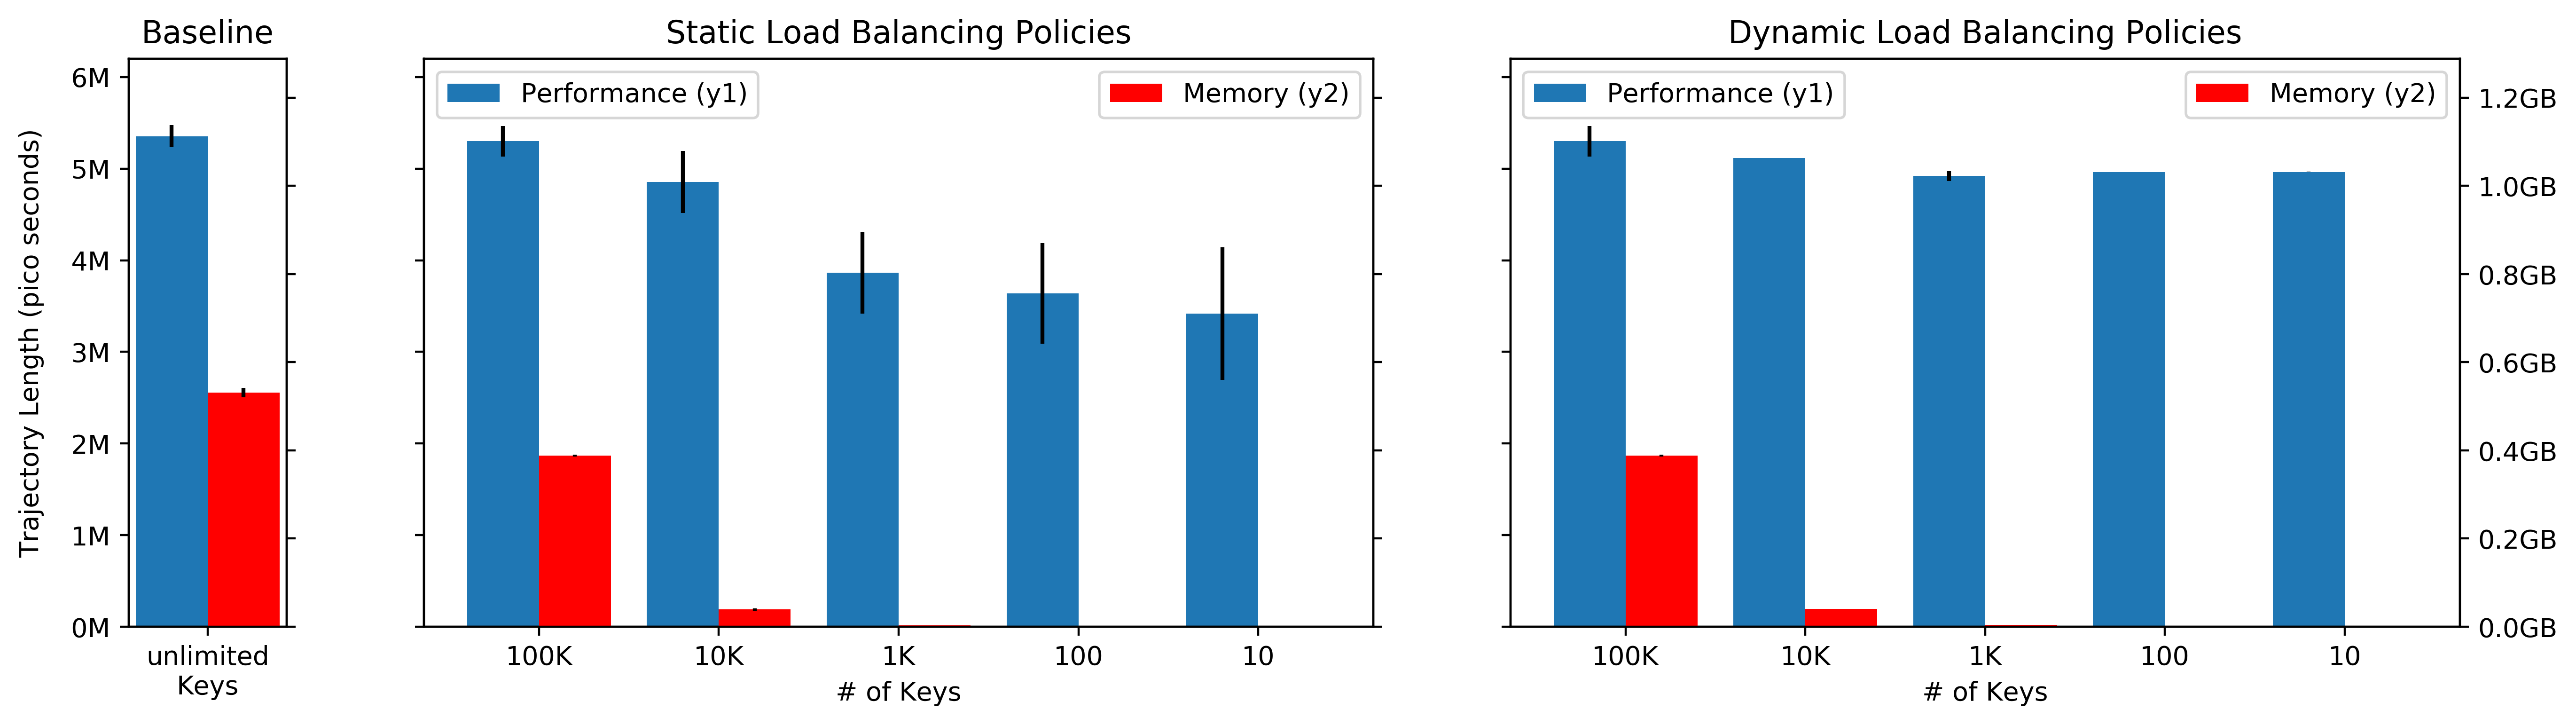
\includegraphics[width=0.5\textwidth]{figures/methodology-tradeoff.png}\\
  \caption{The optimal cache size must strike a balance between performance and
  resoure utilization. Here we show the trade-off for a static load balancing
  policy that evicts keys when the cache reaches a certain size. For this
  configuration, a 100K key cache has the best performance/utilziation, despite
  the keyspace being 250K keys. \label{fig:methodology-tradeoff}}
\end{figure}

\subsection{Contribution 3: The Need for Dynamic Load Balancing Policies}
Why doesn't 1 policy fit all?
\begin{itemize}
  \item keyspace gets less active
  \item beginning: levelDB can't handle it
  \item end: levelDB can handle it
\end{itemize}


\begin{enumerate}
  \item fix DB size to 4GB
  \item trajectory default (1M  and 100K)
  \item trajectory with naiive balancer
\end{enumerate}


\begin{itemize}
  \item Mantle (approach/API) to explore dynamic load balancing policies
  \begin{itemize}
    \item quantifies effect of load balancing
    \item formalized effective FS balancers
    \item debugging tool 
  \end{itemize}
  \item HXHIM is a good fit because it has migration mechanisms for load balancing
  \begin{itemize}
    \item bulk operations (\texttt{put/get()})
    \item key partitioners
    \item secondary indices
  \end{itemize}
  \item we need a way to learn these regimes
  \begin{itemize}
    \item Figure~\ref{keyspace-regimes-4hr} shows the same phases as 100K but that the timestamps affected by delay
  \end{itemize}
\end{itemize}

% What is Mantle?
Mantle is an API that lets admnistrators control file system metadata load
balancing. Mantle speeds up file systems by making metadata access faster,
leveraging the fact that file system metadata IO imposes small and frequent
accesses on the underlying storage system. Since data IO does not scale like
metadata IO~\cite{roselli:atec2000-FS-workloads}, finding optimal ways to
measure, migrate, and partition metadata load is a relatively new field, but
has been shown to lead to large performance increases and more scalable file
systems~\cite{zheng:pdsw2014-batchfs, grider:pdsw2015-marfs,
ren:sc2014-indexfs, patil:fast2011-giga+, brandt:msst2003-lh}.  Mantle can use
strategies from these papers to control how to distribute or concentrate file
system metadata.

% How does it work?
It was built on CephFS, the file system above Ceph, so it inherits many of
characteristics of the CephFS architecture, like the dedicated metadata cluster
and heartbeat mechanisms shown at the top of Figure~\ref{fig:arch-mantle}.
Each metadata server manages differently sized subtrees of the logical
namespace and migration decisions are made synchronously, every 10 seconds.
CephFS already had the mechanisms for load balancing, namely the ability to
measure the load on a subtree, to migrate subtrees, and to partition subtrees
into smaller subtrees, but it had hard-coded, ad-hoc policies for guiding the
migrations.  Mantle reads user-defined policies written in Lua and returns
decisions for how load should be migrated given the state of the cluster and
the behavior of the workload. The hooks in Figure~\ref{fig:arch-mantle} show
where CephFS calls out to the Mantle library to make decisions. While the
decisions were made by Mantle, CephFS used its internal mechanisms to do the
load balancing.

% The actual policies
The Mantle paper implemented three balancers and tested them under
metadata-intensive workloads. The Greedy Spill balancer, which was based
on~\cite{patil:fast2011-giga+}, sheds have its load aggressively when there are
avaiable servers. Part of the Lua code for implementing this balancer is shown
in~\ref{fig:arch-mantle-example}.  The Fill and Spill balancer, which was based
on~\cite{pai:asplos1998-lard} sheds a fraction of the load only when the server
is overloaded. Finally, the Adaptable balancer, which was based
on~\cite{weil:sc2004-dyn-metadata, weil:osdi2006-ceph}, sheds a fraction of the
load frequently.

% What is the status?
It was merged\footnote{https://github.com/ceph/ceph/pull/5155} and is starting
to get users who are frustrated with the hard-coded load balancing policies
that are shipped with CephFS. It was re-implemented using the ``programmable
storage" approach~\cite{sevilla:eurosys17} to reduce lines of code for doing
things like versioning and distributing balancer version.  Although Mantle is
heavily integrated the daemons that compose an Ceph cluster, using Ceph's
naming conventions and internal libraries like Ceph's version of protocol
buffers, there is no reason that it cannot be extracted.

\begin{figure}[tb]
  \noindent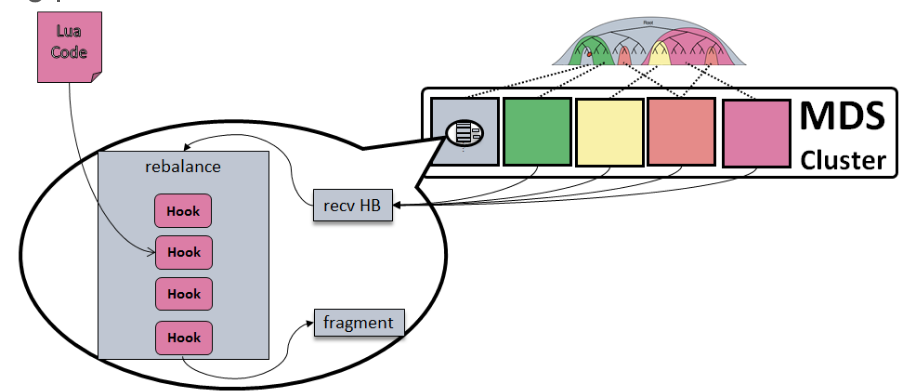
\includegraphics[width=19pc,angle=0]{figures/arch-mantle.png}\\
  \caption{The Mantle API lets adminstrators control load balancing by
  changing the poicies for how to distribution or concentrate file system
  metadata. It was merged into CephFS and inherits many aspects of that
  architecture. Although it has the load balancing structure and logic from
  CephFS (gray boxes), the actual API is not dependent on that code base.}
  \label{fig:arch-mantle}
\end{figure}
\begin{figure}[tb]
  \noindent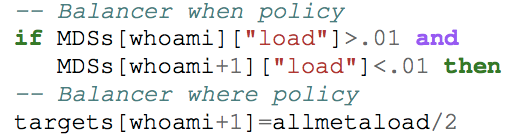
\includegraphics[width=19pc,angle=0]{figures/arch-mantle-example.png}\\
  \caption{The Greedy Spill balancer written in Lua using the Mantle API.}
  \label{fig:arch-mantle-example}
\end{figure}

\subsection{Contribution 4: Machine Learning Keyspace Activity}

We can't find the optimal keypsace size for every permuation, finding the key threshold changes with
\begin{itemize}
  \item number of nodes
  \item size of delay
\end{itemize}


%\begin{itemize}
%  \item C bindings for Mantle
%\end{itemize}
%
%\subsection{Pluggable Interfaces}
%
%\begin{figure}[tb]
%  \noindent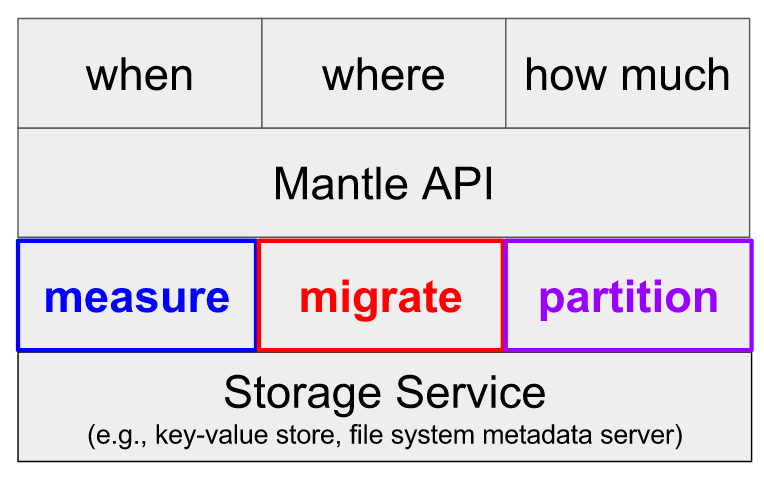
\includegraphics[width=19pc,angle=0]{figures/mantle-pluggable-interfaces.png}\\
%  \caption{The storage service must: \textcolor{blue}{\textbf{measure}}
%  resource usage, \textcolor{red}{\textbf{migrate}} resources, and
%  \textcolor{purple}{\textbf{partition}} resources. }
%  \label{fig:mantle-pluggable-interfaces}
%\end{figure}
%
%\subsubsection{Measure}
%
%The metrics measured should help the system decide ``when" to migrate server
%load. They should:
%
%\begin{itemize}
%  \item tell us about the state of the server or cluster
%  \item provide some value of load, so we can partition/send it
%\end{itemize}
%
%In Ceph: global and local metrics ({\it e.g.}, CPU utilization, file system operation counts) \\
%
%In HXHIM: ???\\
%
%\subsubsection{Migrate}
%
%In Ceph: \texttt{export\_dir()}
%
%In HXHIM: \texttt{mdhimBPut()}, \texttt{mdhimBGet()}, ``adjusting ... keys" ???
%
%\subsubsection{Partition}
%
%In Ceph: subtrees and directory fragments
%
%In HXHIM: secondary indices, cursor types, bul operations
